\chapter*{Anhang}
\label{sec:Anhang}

\section*{Aufgabenstellung}

\section*{Interviews}

\section*{Assessment}

\section*{Projektplan, Protokolle}

\section*{Übersichtausschnitt der Auftragsaufteilung}

\section*{Commit History}

\newpage
\section*{Aufgabe a: Berechnung AP Transistorschaltung}
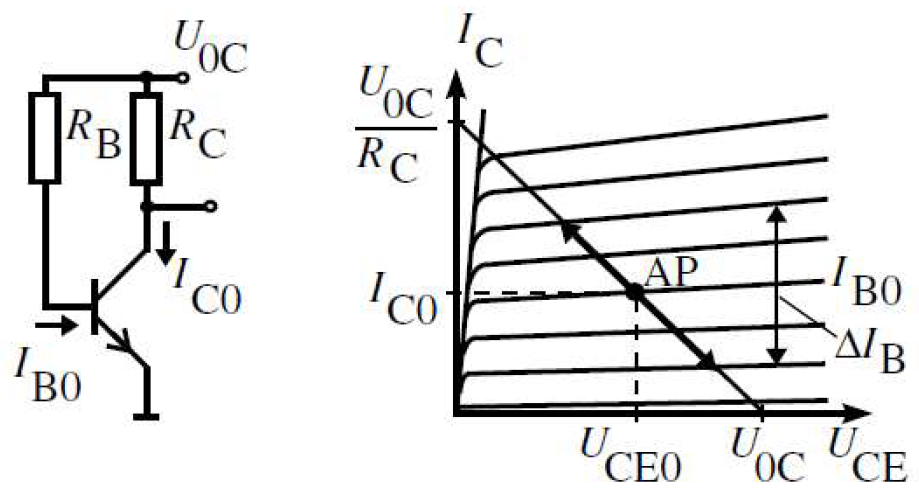
\includegraphics[width=1\textwidth]{images/emitterStufe.png}

Die Speisung VDD(U0C) sei 5V

\begin{enumerate}
\item Wie gross wird der Kollektorstrom IC0 im Arbeitspunkt, wenn die Arbeitspunkt-Spannung
UCE0=VDD/2 betragen soll?
\item Wie gross wird der Basisstrom IB0 für den Arbeitspunkt, wenn Sie einen npn-Transistor zur Verfügung haben und dieser genau den mittleren Stromverstärkungsfaktor hFE aufweist?
\item Wie gross wird die zu erwartende Basis-Emitter-Spannung VBE0 bei Ihrem Arbeitspunkt?
\end{enumerate}

\newpage
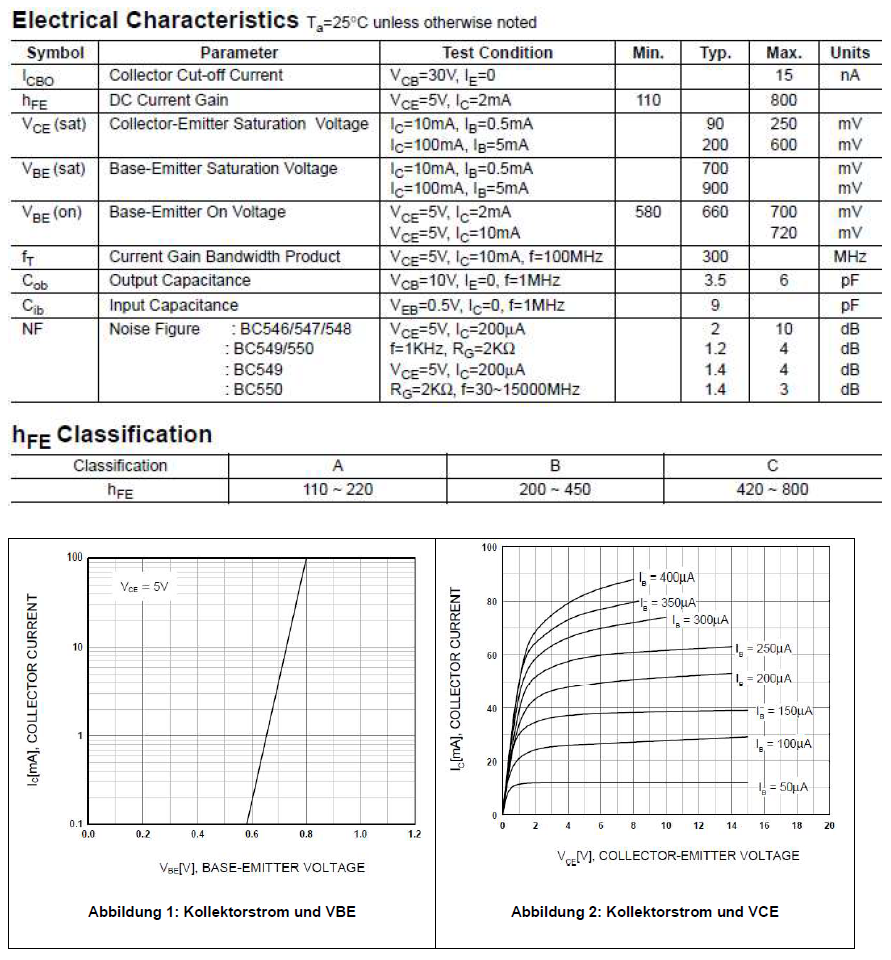
\includegraphics[width=1\textwidth]{images/datasheetBC547.png}
\newpage
\section*{Aufgabe b: Berechnung Operationsverstärkerschaltung T0454}
Gegeben ist folgende Schaltung (T0454) eines Operationsverstärkers mit geschalteten Widerständen

\includegraphics[width=1.2\textwidth]{images/opAmp.png}

Der Opamp sei ideal, d.h. er habe unendliche Verstärkung und Eingangswiderstand,keine Offsetspannung. 
Die Schalter S2, S1 und S1 sind ideal, d.h. es fliesst kein Strom, wenn sie offen sind und es fällt keine Spannung ab, wenn sie geschlossen sind.

Schalterstellung: S2, S1 und S0 geschlossen; Vin1 = 0V, Vin2 = 1V

Für unsere Anwendung soll Vout -1.75 Volt und If 1.75 mA betragen, wobei R2 = 1kOhm, R1 = 2kOhm und R0 4kOhm beträgt.

Wie gross muss Rf sein?
\newpage
\section*{Aufgabe c: Beantwortung E-Mail}
From: pirmin.meier@company.ch\\
To: peter.hasler@company.ch\\

Hallo lieber Peter,\\\\
hiermit sende ich, wie angekündigt, die von Dir so dringend benötigten Informationen. 
Bezüglich der Weiterentwicklung im Bereich der Abteilung Forschung und Entwicklung kann ich Dir folgendes mitteilen. Ich habe mit dem Bereichsleiter T\&E unserer Division gestern ein intensives Gespräch darüber geführt. Mit Sicherheit konnte er mir auch noch nicht viel bestätigen, was aber schon feststeht und sich sicher nicht mehr ändern wird, ist folgendes: Die jetzigen Forschung und Entwicklung Räumlichkeiten werden aufgegeben und ein neues, grösseres Labor am bestehenden Firmengebäude angebaut. Dieser Anbau dürfen wir aber frühestens 2022 erwarten. Die jetzigen zur Verfügung stehenden Messmittel werden zum grossen Teil ersetzt werden, wir werden neue Digital Signal Analyzer und Kathodenstrahloszilloskope mit sechs Kanälen erhalten. Die jetzigen werden, beginnend Ende 2017 etappenweise ersetzt. Genauere Informationen dazu später. Bezüglich dem personellen Ausbau von unserem Team ist momentan eine Personalsteigerung zwischen 15-25\% in Diskussion. Diese Personen werden, beginnend 2018 rekrutiert und in die Abteilung eingegliedert.
Um noch Deine Frage wegen des zu verwendenden Transistors für die Emitterstufe (Schaltung T0455) zu beantworten, ich denke ein off-the-shelf BC547 wird dazu locker reichen. \\
Was ich nun von Dir noch benötige sind folgende Informationen:
Wie gross ist der Feedback-Widerstand des Op-Amp der Schaltung T0454?
Wann genau wirst Du im Herbst deinen WK leisten, damit ich die Personalplanung anpassen kann?
Wie ist der genaue Arbeitsstand im Gerdo-Projekt?
Wie viel Zeit hast Du in etwa aufgewendet, um den Messbericht von Pavel zu korrigieren? Ich brauche diese Angabe für die zukünftige Planung.\\\\
Vielen Dank für Deine Antwort\\\\
Gruss Pirmin

Pirmin Meier\\
El. Ing. HTL\\
Abteilungsleiter F \& E\\
The Company AG\\
6300 Zug\\
Switzerland
   
\textbf{Messbericht Schaltungsteil T0453} Verstärkerschaltung 20.04.17

Der Schaltung vom Schaltungsteil T0453 wurde von mir (Pavel Datsyuk) am 20.04.17 mit Umgebungsbedingungen normal (22 Grade Celsius, 60 Prozentes relativer Luftfeuchtigkeiten) augemessen. Der Resultat der Messung ware wie erwartet positiv ausgefallen. Ich haben die Messunge exakt gleich gemacht auch noch einmal bei 
\section*{Aufgabe e: Ausfüllen Kreuzworträtsel}
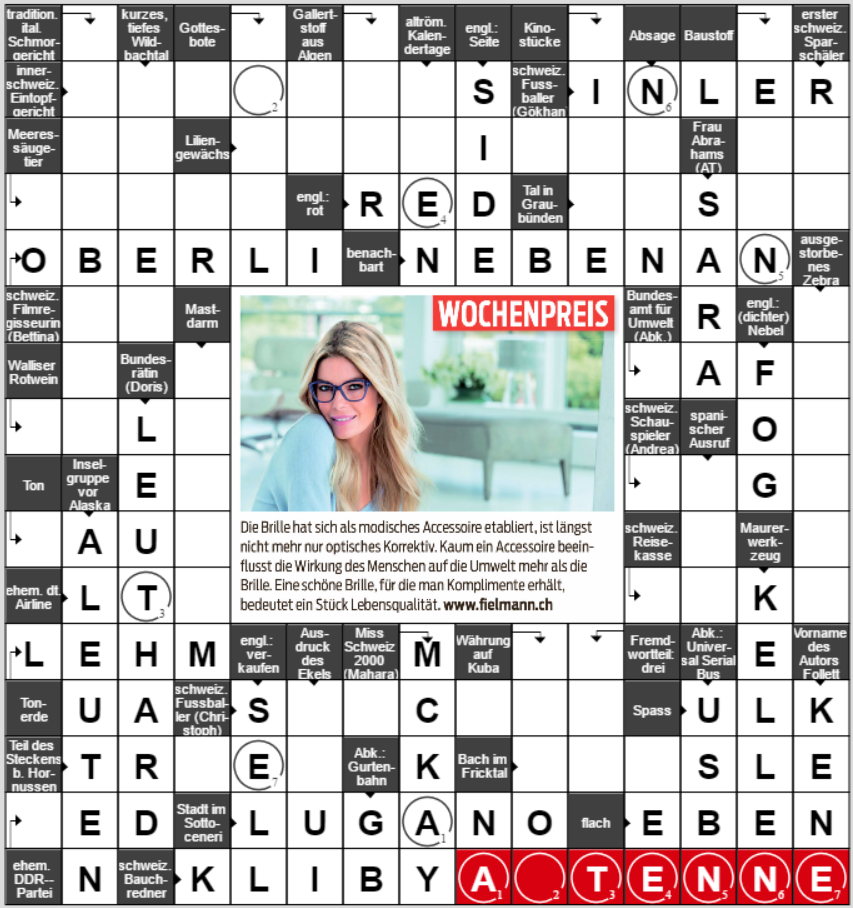
\includegraphics[width=1.2\textwidth]{images/Kreuzwortraetsel.png}
\newpage

\section*{Projektplan, Protokolle}

Datum:03.04.2017\\
Ort: HSR Rapperswil

Teilnehmer: Steve Gerome Kamga, Pascal Horat, Gökhan Kaya\\
Sitzungsleiter: Pascal Horat

Thema: Projektauftrag definieren und verstehen
\begin{enumerate}

\item Ablauf und Aufgabeplanung, Eröffnung der Sitzung 

\item  Verteilung der Aufgaben während der Sitzung
\begin{itemize}
\item Gerome: Sitzungsprotokole
\item Gökhan: Schreiben
\item Pascal: Schreiben 
\end{itemize}

\item Kontext des Projekts definieren un mögliche Fragen zum Projektsbeginn erklären.

\item Mögliche Probleme und Schwierigkeiten erwahnen

\item Regeldokument erstelen : es geht darum, allgemeiner Regeln festzulegen, welche für die Teamarbeit als verbinlich gelten.

\item Projektziele festlegen und Teamrolle gemäss Teamreview 2 beschreiben.

\item Mögliche voraussetzung für einen erfolreichen Projektmanagement definieren

\item Benötigte Literatur: HSR Projektauftrag.docx   

\item Zusammenfassung

\end{enumerate}

Nächste Sitzung: 13.04.2017




\newpage

\section*{Projektplan, Protokolle}

Datum:13.04.2017\\
Ort: HSR Rapperswil

Teilnehmer: Steve Gerome Kamga, Pascal Horat, Gökhan Kaya\\
Sitzungsleiter: keiner

Thema: Klärung der Aufgabenstellung
\begin{enumerate}

\item Ablauf und Aufgabeplanung, Eröffnung der Sitzung 

\item  Verteilung der Aufgaben während der Sitzung
\begin{itemize}
\item Gerome: Sitzungsprotokole
\item Gökhan: Interviewleitfaden erstellen
\item Pascal: MS-Projekt
\end{itemize}

\item GrobePlanung mit Microsoft Projekt erstellen: Damit jeder von uns immer immer auf das Projekt zugreifen kann.

\item Detailplanung erstellen

\item Baseline erstellen und als .pdf speichern

\item Interviewleitfaden erstellen: vorhandener Fragekatalog mit Fragekatalog von Dozent erweitern, Raster für Koordinaten des Befragten erstellen, Frage hinzufügen ob Befragter genannt werden will.

\item Latex-Vorlage Projektbericht organisieren

\item Benötigte Literatur: 

\item Zusammenfassung

\end{enumerate}

Nächste Sitzung: 19.04.2017

\newpage
\section*{Projektplan, Protokolle}

Datum:19.04.2017\\
Ort: HSR Rapperswil

Teilnehmer: Steve Gerome Kamga, Pascal Horat, Gökhan Kaya\\
Sitzungsleiter: keiner

Thema: Plannung und Vorgehen des Interviews (1)

\begin{enumerate}

\item Ablauf und Aufgabeplanung, Eröffnung der Sitzung 

\item  Verteilung der Aufgaben während der Sitzung
\begin{itemize}
\item Gerome: Sitzungsprotokole
\item Gökhan: Internet Suche
\item Pascal: Antwortformular schreiben
\end{itemize}

\item	Projektbericht Template erstellen

\item  interviewleitfaden herstellen:  Mit Hilfe internets zehn Schlüsselkompetenzen auswählen.

\item 	interviewPartner für Beschaffung der Kernkompetenzen notieren: Jeder notiert sich 3 mögliche Partner, die er kontaktieren könnte. damit wir   sicherstellen können, dass jeder am Schluss Kontakt mit ca. 2 Partnern hatte.

\item 	Terminvorschlag mit mögliche Interviewpartner festlegen:  Die Termine sind in unserem Auftragsdokument in Excel unter Tab «Projektpartner» zu notieren.

\item	Antwortformulare Einfordern : Formulare mit Namen der befragten Person beschriften und unter OneDrive/TKI /ProjektAC/Befragung abspeichern.


\item Latex-Vorlage Projektbericht organisieren

\item Benötigte Literatur: Simon 2002   \cite{simon2002entwicklung}

\item Zusammenfassung

\end{enumerate}

Nächste Sitzung: 05.05.2017

\newpage
\section*{Projektplan, Protokolle}

Datum:05.05.2017\\
Ort: HSR Rapperswil

Teilnehmer: Steve Gerome Kamga, Pascal Horat, Gökhan Kaya\\
Sitzungsleiter: keiner

Thema: Auswertung der Interviews

\begin{enumerate}

\item Ablauf und Aufgabeplanung, Eröffnung der Sitzung 

\item  Verteilung der Aufgaben während der Sitzung
\begin{itemize}
\item Gerome: Sitzungsprotokole
\item Gökhan: Grafische Darstellung der Kernkompetenzen
\item Pascal: Projektbericht weiter schreiben
\end{itemize}

\item	Projekt anpassen gemäss plan.


\item 	Übersichtsdokument der Kompetenzen erstellen :In diesem Dokument sollten alle Antworten der Formulare eingetragen und dann ausgewertet werden. Dieses Dokument wird optimalerweise direkt in Projektbericht verfasst.

\item 	Kernkompetenzen ermitteln.

\item 	An Projektbericht weiter schreiben

\item Benötigte Literatur: Simon 2002   \cite{simon2002entwicklung}

\item Zusammenfassung

\end{enumerate}

Nächste Sitzung: 14.05.2017

\newpage
\section*{Projektplan, Protokolle}

Datum:14.05.2017\\
Ort: HSR Rapperswil

Teilnehmer: Steve Gerome Kamga, Pascal Horat, Gökhan Kaya\\
Sitzungsleiter: keiner

Thema: überlegung über Beobachtungsinstrument
\begin{enumerate}

\item Ablauf und Aufgabeplanung, Eröffnung der Sitzung 

\item  Verteilung der Aufgaben während der Sitzung
\begin{itemize}
\item Gerome: Sitzungsprotokole
\item Gökhan: Aufgabe zum lernbereitschaft entwickeln
\item Pascal: Aufgabe zur Selbstmanagement entwickeln
\end{itemize}


\item  Die wichtigsten Kernkompetenzen selektieren:
\begin{itemize}
\item Analytisches und systematisches Denken
\item Lernbereitschaft und Lernfähigkeit
\item Selbstmanagement und Selbstorganisation 
\end{itemize}

\item mögliche Ideen zum Beobachtungsinstrument vorschlagen: es geht darum zwei übungen zu entwickeln,  mit denen sich die fünf von uns gewählten Kernkompetenzen herauskristalisiernen lassen

\item Erzeugung Von Übungen zum Testen der Kernkompetenzen

\item Powerpoint Vorlage für die Präsentation vorbereiten	

\item Probanten für den Test der Kernkompetenzen auswählen


\item Benötigte Hilfsmittel: Internet 

\item Zusammenfassung

\end{enumerate}

Nächste Sitzung: 19.05.2017

\newpage
\section*{Projektplan, Protokolle}

Datum:19.05.2017\\

Ort: HSR Rapperswil

Teilnehmer: Steve Gerome Kamga, Gökhan Kaya\\

Sitzungsleiter: keiner

Thema: Erstellung der Projektpräsentation
\begin{enumerate}

\item Ablauf und Aufgabeplanung, Eröffnung der Sitzung 

\item  Verteilung der Aufgaben während der Sitzung
\begin{itemize}
\item Gerome: Präsentation entwickeln
\item Gökhan: Präsentation entwickeln
\end{itemize}

\item PowerPoint erzeugen und einrichten

\item Präsentation üben


\item Benötigte Literatur: 

\item Zusammenfassung

\end{enumerate}

Nächste Sitzung: 01.06.2017



\newpage
\section*{Projektplan, Protokolle}

Datum:01.06.2017\\
Ort: HSR Rapperswil

Teilnehmer: Steve Gerome Kamga, Pascal Horat, Gökhan Kaya\\
Sitzungsleiter: keiner

Thema: Bewertung der Probanten
\begin{enumerate}

\item Ablauf und Aufgabeplanung, Eröffnung der Sitzung 

\item  Verteilung der Aufgaben während der Sitzung
\begin{itemize}
\item Gerome: Sitzungsprotokole
\item Gökhan: Interpretation der Ergebnissen
\item Pascal: Interpretation der Ergebnissen
\end{itemize}

\item Resultate der einzelnen Probanten analysieren, interpretieren und schön darstellen 		

\item 	Projektauftrag weiter schreiben

\item 	Bewertung der Ergebnissen von Beobachtungsinstrument


\item Benötigte Literatur

\item Zusammenfassung

\end{enumerate}

Nächste Sitzung: 07.06.2017

\newpage
\section*{Projektplan, Protokolle}

Datum:07.06.2017\\
Ort: HSR Rapperswil

Teilnehmer: Steve Gerome Kamga, Pascal Horat, Gökhan Kaya\\
Sitzungsleiter: keiner

Thema: Projektbericht fertigstellen
\begin{enumerate}

\item Ablauf und Aufgabeplanung, Eröffnung der Sitzung 

\item  Verteilung der Aufgaben während der Sitzung
\begin{itemize}
\item Gerome: Sitzungsprotokole
\item Gökhan: Auswertung der Übungen schreiben
\item Pascal: Bericht erweitern
\end{itemize}

\item Bewertungsergebnisse zur Lernbereitschaft und Lernfähigkeit

\item Verfassung der Übungsauswertung, Kapitel 3 (Klärung Projektauftrag)  sowie Zusammenfassung im Projektbericht 

\item Auswertung Assesment in Projektbericht

\item Interview ausbauen und Reflexion Verfassen

\item Schlussfolgerungen, Ausblicke und Empfehlungen verfassen 

\item Zusammenfassung

\end{enumerate}

Nächste Sitzung: 8.06.2017

\newpage

\section*{Übersichtausschnitt der Auftragsaufteilung}

%\begin{tabular}{ | l | l | l |}
 %\begin{tabular}{ | p{7cm} | p{4cm} | p{2cm} |}
 \begin{longtable}{ | p{7cm} | p{4cm} | p{2cm} |}
   \hline
   \textbf{Auftrag} & \textbf{Verfasser} & \textbf{Zeit[min]}   \\
   \hline  		
    Microsoft Project einrichten & Gerome & 60 \\ \hline
    Detailplanung erstellen & Pascal & 180 \\ \hline
    Baseline erstellen  & Pascal & 30 \\ \hline
    Interviewleitfaden erstellen& Gökhan,Gerome & 180 \\ \hline
    LaTeX-Vorlage Projektbericht organisieren & Pascal, Gökhan & 100 \\ \hline
    Lernbilanz 2 & Pascal, Gerome,Gökhan & - \\ \hline
    lernbilanz 3 & Pasacl, Gerome,Gökhan & - \\ \hline
    Projektbericht Template erstellen & Gökhan & 120 \\ \hline
    Partner für Beschaff. Kernkomp. notieren & Pascal,Gerome,Gökhan & 30 \\ \hline
    Projektplan anpassen gemäss Angaben & Pascal & 120 \\ \hline
    Termine Interviewpartner festlegen & Pascal, Gerome, Gökhan & 30 \\ \hline
    Formulare versenden & Pascal, Gerome Göhkan & 15 \\ \hline
    Antwortformulare Einfordern & Pascal, Gerome, Gökhan & 10 \\ \hline
    Übersichtsdok. Kompetenzen erstellen & Gökhan & 60 \\ \hline    
    Kernkompetenzen ermitteln & Gerome,Gökhan & 10 \\ \hline   
    an Projektbericht schreiben & Gökhan & 90 \\ \hline   
    Punkt c im File AuftragAC\_ersteLektion.png erledigen & Pascal & 20 \\ \hline    
    Aufgabe entwickeln oder finden um die Kernkompetenz Lernbereitschaft zu testen  & Pascal & 120 \\ \hline   
    Aufgabe entwickeln oder finden um die Kernkompetenz Selbstmanagement zu testen  & Gökhan & 120 \\ \hline  
    Teamsitzungsprotokolle erstellen & Gerome & 100 \\ \hline    
    Analyse Projektauftrag in main.tex einbringen, Vorlage in HSR\_Projektauftrag.docx & Gerome, Gökhan & 20\\ \hline   
    Übersicht erstellen wer wie viel Zeit für was investiert hat im Projekt TKI & Gerome & 60\\ \hline   
    Commit-History in 06vorgehen.tex schön formatieren & Gerome & 30 \\ \hline 
    Auswertung der Übung in Projektbericht verfassen  & Pascal, Gökhan & 480 \\ \hline   
Auswertung des Assessments in Projektbericht verfassen & Pascal, Gökhan & 200 \\ \hline  
Zusammenfassung auf Seite 2 in Projektbericht verfassen     & Pascal & 30 \\ \hline   
Commit-History aus Git extrahieren und in Latex erweitern, in Anhang von Projektbericht verschieben     & Gerome & 30 \\ \hline
 Verzeichnisse (Kapitel 1) einfügen in Projektbericht    & Pascal & 20 \\ \hline  
 Einleitung erweitern    & Pascal & 90 \\ \hline   
 Kapitel 3 verfassen (Klärung Projektauftrag)    & Pascal & 90 \\ \hline
 Formattierung Projektbericht verbessern (inkl. Unterschriften in Kapitel 4)    & Pascal, Gökhan & 120 \\ \hline  
 Kapitel 7 Interview ausbauen  & Pascal, Gökhan & 200 \\ \hline   
 Kapitel 11 Reflexion verfassen & Pascal, Gökhan &  \\ \hline    
 Kapitel 12 Schlussfolgerungen, Ausblicke und Empfehlungen    verfassen & Pascal, Gökhan & 60 \\ \hline  
 Erklärung Urheberschaft einfügen & Pascal & 30 \\ \hline   
 Anhang in Projektbericht erweitern & Gerome & 30 \\ \hline     
 Tabelle Übersichtausschnitt der Auftragsaufteilung in Projektbericht aktualisieren anhand \_Aufträge.xlsx    & Gerome & 30 \\ \hline    
     &  &  \\ \hline  
     
%\end{tabular}
\end{longtable}
     
\newpage

\section*{Commit History} \label{sec:comhist}
 


%AB HIER KANN JEROME FORMATIEREN
SteveGerome, Thu Jun 8 14:41:41 2017 +0200 : übersichtausschnitt Auftragsaufteilung 2 \\
SteveGerome, Thu Jun 8 13:38:13 2017 +0200 : übersichtausschnitt Auftragsaufteilung 1 \\
SteveGerome, Thu Jun 8 08:27:47 2017 +0200 : übersichtausschnitt Auftragsaufteilung \\
kaya, Wed Jun 7 15:45:05 2017 +0200 : Bewertung fertiggestellt. Noch kommentieren \\
Corumh, Wed Jun 7 14:35:31 2017 +0200 : Alles zusammen kompiliert \\
kaya, Wed Jun 7 14:28:50 2017 +0200 : Merge branch 'master' of https://github.com/cruis1/tki Konflikt \\
kaya, Wed Jun 7 14:28:35 2017 +0200 : Ein Teil der Bewertung geschrieben \\
Corumh, Wed Jun 7 14:24:53 2017 +0200 : Auswertung Assessment weitergeschrieben \\
Corumh, Wed Jun 7 12:00:57 2017 +0200 : Auswertung der Übung 2 weitergeschr. \\
Corumh, Wed Jun 7 11:08:15 2017 +0200 : Auswertung des Assessments weitergeschr. \\
Corumh, Wed Jun 7 10:49:07 2017 +0200 : Auswertung des Assessments angefangen \\
Corumh, Wed Jun 7 09:37:18 2017 +0200 : Bewertungsanmerkungen Probanden angefangen \\
Corumh, Wed Jun 7 09:15:48 2017 +0200 : Bewertungstabellen Probanden fertig \\
Corumh, Tue Jun 6 19:47:35 2017 +0200 : Protokolle angepasst \\
SteveGerome, Tue Jun 6 19:38:49 2017 +0200 : Sitzungsprotokolle verbessert 1 \\
SteveGerome, Tue Jun 6 19:32:49 2017 +0200 : Sitzungsprotokolle verbesssert \\
SteveGerome, Tue Jun 6 15:20:25 2017 +0200 : Commit History form. beendet \\
Corumh, Tue Jun 6 15:06:20 2017 +0200 : Bewertung Probanden Selbstmanagement gem. \\
Corumh, Tue Jun 6 13:28:31 2017 +0200 : Bewertung Probanden weitergeschr. \\
Corumh, Tue Jun 6 13:05:02 2017 +0200 : Bewertung Probanden angefangen \\
Corumh, Tue Jun 6 12:25:31 2017 +0200 : Einleitung angepasst \\
Corumh, Tue Jun 6 12:20:58 2017 +0200 : gitignore angepasst \\
Corumh, Tue Jun 6 12:16:57 2017 +0200 : gitignore angepasst \\
Corumh, Tue Jun 6 12:14:32 2017 +0200 : gitignore angepasst \\
Corumh, Tue Jun 6 11:58:05 2017 +0200 : Ablauf Assessment beschr. \\
SteveGerome, Tue Jun 6 11:54:51 2017 +0200 : Commit History form. beendet \\
SteveGerome, Tue Jun 6 11:34:53 2017 +0200 : Commit History form. weiter verbe. \\
kaya, Tue Jun 6 11:25:39 2017 +0200 : Merge branch 'master' of https://github.com/cruis1/tki Merge \\
kaya, Tue Jun 6 11:25:24 2017 +0200 : Mainfile Projektauftrag hinzugefügt \\
Corumh, Tue Jun 6 11:22:24 2017 +0200 : Merge branch 'master' of https://github.com/cruis1/tki \\
Corumh, Tue Jun 6 11:21:39 2017 +0200 : Commit History Formattierung verb. \\
kaya, Tue Jun 6 11:21:37 2017 +0200 : Filevorlage Projektauftrag erstellt \\
SteveGerome, Tue Jun 6 11:15:50 2017 +0200 : Commit History form. verb. \\
SteveGerome, Tue Jun 6 11:09:43 2017 +0200 : trying \\
SteveGerome, Tue Jun 6 11:08:57 2017 +0200 : trying \\
SteveGerome, Tue Jun 6 11:05:35 2017 +0200 : trying \\
SteveGerome, Tue Jun 6 11:02:12 2017 +0200 : trying \\
Corumh, Tue Jun 6 10:54:42 2017 +0200 : gitignore Assessment erstellt \\
kaya, Tue Jun 6 10:30:00 2017 +0200 : Commit history hinzugefügt \\
kaya, Thu Jun 1 16:15:20 2017 +0200 : Diverse Änderungen im Abschnit Teamgrundlagen und Vorgehen \\
kaya, Thu Jun 1 15:32:12 2017 +0200 : Merge branch 'master' of https://github.com \\
kaya, Thu Jun 1 16:15:20 2017 +0200 : Diverse Änderungen im Abschnitt Teamgrundlagen und Vorgehen \\
kaya, Thu Jun 1 15:32:12 2017 +0200 : Merge branch 'master' of https://github.com/cruis1/tki merge \\
kaya, Thu Jun 1 15:32:03 2017 +0200 : Teil Vorgehen überarbeitet \\
Corumh, Thu Jun 1 15:25:52 2017 +0200 : Übung Selbstmanag. mitzut. Infos fertigg. \\
kaya, Thu Jun 1 14:44:34 2017 +0200 : Merge branch 'master' of https://github.com/cruis1/tki böö \\
kaya, Thu Jun 1 14:44:23 2017 +0200 : Teil Vorgehen geschrieben \\
Corumh, Thu Jun 1 14:42:44 2017 +0200 : Übung Selbstmanag. mitzut. Infos angef. \\
Corumh, Thu Jun 1 13:58:12 2017 +0200 : Übung Selbstmanag. verfeinert \\
Corumh, Thu Jun 1 13:19:40 2017 +0200 : Merge branch 'master' of https://github.com/cruis1/tki \\
Corumh, Wed May 31 17:51:22 2017 +0200 : Übung Selbstmanag. alle Aufgabe fertig \\
kaya, Wed May 31 16:02:27 2017 +0200 : Teil Klärung der Aufgabenstellung angefangen \\
kaya, Wed May 31 15:31:15 2017 +0200 : Merge branch 'master' of https://github.com/cruis1/tki kei ahnig was lauft \\
kaya, Wed May 31 15:28:27 2017 +0200 : Fragetext korrigiert \\
Corumh, Wed May 31 15:22:57 2017 +0200 : Merge branch 'master' of https://github.com/cruis1/tki \\
Corumh, Wed May 31 15:22:32 2017 +0200 : Übung Selbstmanag. E-Mail-Aufgabe fertig \\
kaya, Wed May 31 15:12:52 2017 +0200 : Einleitung korrigiert \\
kaya, Wed May 31 14:46:12 2017 +0200 : Kapitel Teamgrundlagen geschrieben. Achtung: Kann fehler verursachen beim kompilieren \\
kaya, Wed May 31 12:17:54 2017 +0200 : Vorbereitungen für Teamvertrag img ordner hinzugefügt \\
Corumh, Wed May 31 12:16:43 2017 +0200 : Übung Selbstmanag. Kreuzwortraetsel fertig \\
kaya, Wed May 31 11:51:52 2017 +0200 : Erster Teil der Einleitung \\
Corumh, Wed May 31 11:48:57 2017 +0200 : Übung Selbstmanag. Messbericht fast fertig \\
kaya, Wed May 31 10:56:55 2017 +0200 : kleine korrekturen \\
Corumh, Wed May 31 10:49:15 2017 +0200 : Übung Selbstmanag. Messbericht weitergeschr. \\
kaya, Wed May 31 10:40:43 2017 +0200 : Merge branch 'master' of https://github.com/cruis1/tki testmerge \\
kaya, Wed May 31 10:40:15 2017 +0200 : Tabelle korrigiert \\
Corumh, Wed May 31 10:39:52 2017 +0200 : Übung Selbstmanag. Messbericht angef. \\
Kaya, Tue May 30 20:30:33 2017 +0200 : Diverse Tabellen hinzugefügt \\
Kaya, Tue May 30 19:56:43 2017 +0200 : Viele Korrekturen und weitere Arbeiten \\
kaya, Tue May 30 18:11:52 2017 +0200 : Teil Test1 hinzugefügt \\
Corumh, Tue May 30 16:27:24 2017 +0200 : Übung Selbstmanag. Bewertungskriterien weiter beschr. \\
Corumh, Tue May 30 15:19:04 2017 +0200 : Beobachtungsinstr. Selbstmanag. Bewertungskriterien beschr. \\
kaya, Tue May 30 14:47:56 2017 +0200 : nüt \\
Corumh, Tue May 30 14:29:34 2017 +0200 : Beobachtungsinstr. Selbstmanag. Bewertung \\
Corumh, Tue May 30 13:53:05 2017 +0200 : Beobachtungsinstr. Selbstmanag. Aufgaben weiter beschrieben \\
Corumh, Mon May 29 17:14:46 2017 +0200 : Beobachtungsinstr. Selbstmanag. Aufgaben beschrieben \\
Corumh, Mon May 29 16:10:04 2017 +0200 : Beobachtungsinstr. Selbstmanag. Detail beschrieben \\
Corumh, Mon May 29 16:06:30 2017 +0200 : Beobachtungsinstr. Selbstmanag. weiter beschrieben \\
Corumh, Mon May 29 15:56:12 2017 +0200 : Beobachtungsinstr. Selbstmanag. beschrieben \\
Kaya, Thu May 25 20:42:47 2017 +0200 : Korrekturen und weitere Arbeiten \\
Corumh, Sun May 14 16:07:20 2017 +0200 : Projektbericht Fehler behoben \\
kaya, Mon May 8 16:01:52 2017 +0200 : readme update \\
kaya, Mon May 8 16:00:37 2017 +0200 : readme update \\
kaya, Mon May 8 15:52:42 2017 +0200 : korrekturen \\
kaya, Mon May 8 15:40:18 2017 +0200 : Kernkompetenz Auswertung hinzugefügt, Assessmentbericht Interviewteil weitergeschrieben \\
kaya, Mon May 8 14:59:29 2017 +0200 : HILFE file überarbeitet \\
kaya, Mon May 8 14:58:12 2017 +0200 : HILFE file erstellt für die hartnäckige merge konflikt \\
Corumh, Mon Apr 24 16:35:48 2017 +0200 : Projektbericht Referenz Website \\
kaya, Mon Apr 24 16:31:32 2017 +0200 : ksjdksj \\
Corumh, Mon Apr 24 16:26:53 2017 +0200 : Projektbericht Referenz Website \\
Corumh, Mon Apr 24 16:26:05 2017 +0200 : Projektbericht Referenz Website \\
kaya, Mon Apr 24 16:21:51 2017 +0200 : nüt spannends \\
kaya, Mon Apr 24 15:11:00 2017 +0200 : Ordner Projektbericht gelöscht \\
kaya, Mon Apr 24 12:12:08 2017 +0200 : Fragekatalog verbessert 2 \\
kaya, Mon Apr 24 12:05:55 2017 +0200 : Fragenkatalog korrigiert \\
kaya, Wed Apr 19 19:09:19 2017 +0200 : Assessmentbericht template fertig \\
kaya, Wed Apr 19 15:34:54 2017 +0200 : Fragekatalog nachgebessert \\
kaya, Wed Apr 12 21:02:19 2017 +0200 : Fragenkatalog angepasst \\
Corumh, Mon Apr 3 23:26:16 2017 +0200 : TR3 Orthografie korrigiert \\
Corumh, Mon Apr 3 23:02:35 2017 +0200 : TR3 komplett überarbeitet \\
Corumh, Mon Apr 3 20:29:41 2017 +0200 : TR3 Protokoll eingefügt \\
kaya, Mon Apr 3 20:00:33 2017 +0200 : TR3 fast fertig \\
kaya, Mon Apr 3 18:45:59 2017 +0200 : Gruppeneinschätzung fertig \\
kaya, Mon Apr 3 16:48:33 2017 +0200 : TR3 continue \\
Corumh, Mon Apr 3 16:01:09 2017 +0200 : TR3 Web-Pic eingefügt \\
Corumh, Mon Apr 3 15:57:15 2017 +0200 : Merge branch 'master' of https://github.com/cruis1/tki \\
kaya, Mon Apr 3 15:56:59 2017 +0200 : Arbeit... \\
Corumh, Mon Apr 3 14:52:12 2017 +0200 : TR2 Änderig\\
Corumh, Mon Apr 3 14:08:39 2017 +0200 : TR3 Vorlage pagebreak entfernt\\
kaya, Mon Apr 3 14:04:13 2017 +0200 : TR3 vorlage angepasst\\
Corumh, Mon Apr 3 02:27:49 2017 +0200 : TR3 Vorlage Fehler entfernt\\
kaya, Mon Mar 27 16:41:16 2017 +0200 : nichts nennenswertes\\
Corumh, Mon Mar 27 15:50:50 2017 +0200 : TR3 Vorlage angefangen\\
Corumh, Mon Mar 27 12:11:55 2017 +0200 : TR2 in finale Form gebracht\\
kaya, Mon Mar 27 11:08:49 2017 +0200 : pagebreak aenderungen auskommentiert\\
Corumh, Mon Mar 27 01:59:09 2017 +0200 : TR2 zusätzliche Literatur eingefügt\\
Corumh, Mon Mar 27 00:38:32 2017 +0200 : TR2 kompl. überarb. (Rechtschreibef.) und erweitert\\
Corumh, Sun Mar 26 17:45:31 2017 +0200 : TR2 fast fertig\\
Corumh, Sun Mar 26 15:27:03 2017 +0200 : an TR2 weitergearbeitet\\
SteveGerome, Sun Mar 26 15:16:44 2017 +0200 : weitergeschrieben TR2\\
Corumh, Sun Mar 26 14:55:44 2017 +0200 : an TR2 weitergearbeitet, Bilder eingefügt\\
Corumh, Thu Mar 23 14:24:16 2017 +0100 : an TR2 weitergearbeitet, Bilder eingefügt\\
Corumh, Thu Mar 23 14:03:00 2017 +0100 : .rtf gelöscht\\
Corumh, Thu Mar 23 13:59:07 2017 +0100 : .log gelöscht\\
Corumh, Thu Mar 23 13:57:40 2017 +0100 : TR2 Formattierung verschönert und weitergeschrieben\\
Corumh, Thu Mar 23 13:16:42 2017 +0100 : TR2 weitergearbeitet\\
SteveGerome, Wed Mar 22 21:23:31 2017 +0100 : zweiter Commit :-)\\
Corumh, Wed Mar 22 21:18:40 2017 +0100 : einige Korrekturen in TR2\\
SteveGerome, Wed Mar 22 21:15:22 2017 +0100 : erster Commit :-)\\
Corumh, Wed Mar 22 20:27:56 2017 +0100 : neueste Teamreview 2 Version Upload\\
kaya, Wed Mar 22 20:22:35 2017 +0100 : shit happened\\
kaya, Wed Mar 22 20:15:19 2017 +0100 : Selbsteinschätzung bearbeitet\\
Corumh, Wed Mar 22 20:10:43 2017 +0100 : hoffentlich klappts\\
kaya, Wed Mar 22 20:06:50 2017 +0100 : Merge branch 'master' of https://github.com/cruis1/tki\\
kaya, Wed Mar 22 20:06:26 2017 +0100 : Selbsteinschätzung überarbeitet\\
Corumh, Wed Mar 22 20:05:09 2017 +0100 : hoffentlich klappts\\
kaya, Wed Mar 22 19:45:55 2017 +0100 : Merge branch 'master' of https://github.com/cruis1/tki\\
kaya, Wed Mar 22 19:44:30 2017 +0100 : Fremdeinschätzung grob ferig\\
Corumh, Wed Mar 22 19:34:07 2017 +0100 : zum Abgliche\\
Corumh, Wed Mar 22 19:02:33 2017 +0100 : resolve merge error\\
Corumh, Wed Mar 22 18:45:58 2017 +0100 : Teamreview 2 Selbsteinsch. bearb\\
kaya, Wed Mar 22 18:45:31 2017 +0100 : test\\
kaya, Wed Mar 22 18:38:25 2017 +0100 : Merge branch 'master' of https://github.com/cruis1/tki\\
kaya, Wed Mar 22 18:34:32 2017 +0100 : removed Fremdeinschätzung\\
Corumh, Wed Mar 22 18:32:15 2017 +0100 : Teamreview 2 Selbsteinsch. bearb\\
kaya, Wed Mar 22 18:23:28 2017 +0100 : selbsteinschätzung erstellt\\
kaya, Wed Mar 22 17:04:09 2017 +0100 : selbsteinschätzung erstellt\\
Corumh, Tue Mar 21 17:35:53 2017 +0100 : Teamreview 2 weitererstellt, Referenzen funktionieren\\
Corumh, Tue Mar 21 17:32:52 2017 +0100 : Teamreview 2 weitererstellt, Referenzen funktionieren\\
Corumh, Tue Mar 21 13:56:24 2017 +0100 : Teamreview 2 Struktur erstellt, Referenzen funktionieren\\
Corumh, Tue Mar 21 12:09:38 2017 +0100 : Teamreview 2 Template angefangen\\
Corumh, Tue Mar 21 11:30:41 2017 +0100 : Ordnerstruktur geändert und noch mehr aufgeräumt\\
Corumh, Tue Mar 21 11:18:35 2017 +0100 : Ordnerstruktur geändert und aufgeräumt\\
Corumh, Tue Mar 21 11:10:12 2017 +0100 : Upload TR2\\
Corumh, Mon Mar 20 20:12:37 2017 +0100 : Penis\\
Corumh, Mon Mar 20 19:28:05 2017 +0100 : Upload TR2\\
Corumh, Mon Mar 20 16:13:56 2017 +0100 : Upload TR2\\
Corumh, Mon Mar 20 15:07:02 2017 +0100 : Upload TR2\\
Corumh, Mon Mar 20 13:58:25 2017 +0100 : Upload Vorlage TR2\\
Corumh, Mon Mar 20 12:29:35 2017 +0100 : Reflexion Sitzung finalisiert\\
Corumh, Fri Mar 17 17:07:49 2017 +0100 : Reflexion Sitzung erstellt\\
Corumh, Fri Mar 17 16:22:08 2017 +0100 : Traktl. final.\\
Corumh, Thu Mar 16 20:41:02 2017 +0100 : Upload Traktl. akt.\\
Corumh, Thu Mar 16 20:10:54 2017 +0100 : Upload Traktl.\\
Corumh, Thu Mar 16 19:40:46 2017 +0100 : Konflikt bereinige\\
Corumh, Mon Mar 13 20:53:49 2017 +0100 : Reflexion TR1 erstellt\\
kaya, Mon Mar 13 17:19:59 2017 +0100 : Merge branch 'master' of https://github.com/cruis1/tki\\
kaya, Mon Mar 13 17:06:10 2017 +0100 : Name angepasst\\
kaya, Mon Mar 13 17:04:04 2017 +0100 : Name angepasst\\
kaya, Mon Mar 13 17:02:42 2017 +0100 : Name angepasst\\
Corumh, Mon Mar 13 16:46:47 2017 +0100 : Reflexion TR1 erstellt\\
kaya, Mon Mar 13 16:32:36 2017 +0100 : Änderungen an trakdandenliste\\
kaya, Mon Mar 13 16:13:56 2017 +0100 : Trakdandenliste explizit vervollständigt\\
kaya, Mon Mar 13 15:42:03 2017 +0100 : Fragenkatalog fertiggestellt\\
kaya, Mon Mar 13 15:10:35 2017 +0100 : Fragenkatalog Vorlage erstellt\\
kaya, Mon Mar 13 14:31:25 2017 +0100 : Fragenkatalog erstellt\\
Corumh, Mon Mar 13 12:35:32 2017 +0100 : Merge branch 'master' of https://github.com/cruis1/tki\\
Corumh, Mon Mar 13 12:34:18 2017 +0100 : Regeldokument finalisiert\\
Columh, Sun Mar 12 23:49:13 2017 +0100 : Add files via upload\\
kaya, Sun Mar 12 20:20:00 2017 +0100 : trakdandenliste\_vorlage grob fertig\\
kaya, Sun Mar 12 18:50:06 2017 +0100 : trakdandenliste erstellt\\
Corumh, Thu Mar 9 17:49:18 2017 +0100 : Regeldokument erweitert mit Bildern\\
Corumh, Thu Mar 9 10:47:33 2017 +0100 : Regeldokument erweitert\\
Corumh, Tue Mar 7 13:54:55 2017 +0100 : Regeldokument erstellt\\
kaya, Mon Mar 6 16:56:25 2017 +0100 : Aufträge aktualisiert\\
kaya, Mon Mar 6 16:29:39 2017 +0100 : teamreview update\\
kaya, Mon Mar 6 15:29:30 2017 +0100 : teamreview bearbeitet\\
kaya, Mon Mar 6 14:55:55 2017 +0100 : Ordner umbenannt und teamreview erstellt\\
Corumh, Mon Mar 6 14:07:14 2017 +0100 : LaTex Template verbessert\\
Corumh, Mon Mar 6 14:01:18 2017 +0100 : LaTex Template erstellt\\
Corumh, Mon Mar 6 12:02:56 2017 +0100 : LaTex Template angefangen\\
Corumh, Sun Mar 5 20:23:42 2017 +0100 : ToDo angepasst\\
cruis1, Sun Mar 5 00:18:42 2017 +0100 : Delete\_config.yml\\
kaya, Sun Mar 5 00:14:02 2017 +0100 : Merge branch 'master' of https://github.com/cruis1/tki\\
cruis1, Sun Mar 5 00:10:44 2017 +0100 : Delete\_config.yml\\
kaya, Sun Mar 5 00:04:13 2017 +0100 : doodle zu moodle geändert :)\\
cruis1, Sun Mar 5 00:01:11 2017 +0100 : Set theme jekyll-theme-cayman\\
kaya, Sat Mar 4 23:52:00 2017 +0100 : Alle files synchronisiert md file update\\
kaya, Sat Mar 4 23:36:00 2017 +0100 : Links hinzugefügt\\
cruis1, Sat Mar 4 23:31:16 2017 +0100 : Delete new.md\\
kaya, Sat Mar 4 23:09:51 2017 +0100 : edit readme and add new.md s\\
cruis1, Sat Mar 4 22:15:50 2017 +0100 : Initial commit\\
%BIS HIER

%BEFEHL: git log --pretty=format:"%an, %ar : %s"
%BEFEHL evt. besser: git log --pretty=format:"%an, %ad : %s"
%https://git-scm.com/book/tr/v2/Git-Basics-Viewing-the-Commit-History
    
   
